\documentclass[main]{subfiles}

\begin{document}

\begin{definition}
When $z\in\mathbb CP^1$ is a fixed point of an elliptic/parabolic/hyperbolic element in $\Gamma$, we say $z$ is an elliptic/parabolic/hyperbolic point of $\Gamma$
\end{definition}

\subsection{The case of $\Gamma=\SL_2(\mathbb Z)$}

\begin{exercise}
$\SL_2(\mathbb Z)$ is generated by $T=\begin{bmatrix}
1&1 \\
0&1
\end{bmatrix}$ and $S=\begin{bmatrix}
0&-1 \\
1&0
\end{bmatrix}$, the same is true for $\PSL_2(\mathbb Z)$
\end{exercise}

\begin{proof}
Use Euclid's algorithm we can make any matrix upper triangular, $S^2=-I_2$, $T^n=\begin{bmatrix}
1&n \\
&1
\end{bmatrix}$
\end{proof}

\begin{theorem}
Let $\mathcal D=\left\{z\in\mathcal H||z|\geq1,|\operatorname{Re}(z)|\leq\frac{1}{2}\right\}$, $\rho=e^{i\frac{\pi}{3}}$
\begin{center}
\begin{tikzpicture}
\begin{scope}[xshift=-4cm]
\coordinate (1) at ($cos(60)*(1,0)+sin(60)*(0,1)$);\node at (1) [above right] {$\rho=e^{i\frac{\pi}{3}}$};
\coordinate (2) at ($cos(120)*(1,0)+sin(120)*(0,1)$);\node at (2) [above left] {$\rho^2$};
\filldraw[gray,opacity=0.5] ($(1)+(0,2)$)--(1)--(2)--($(2)+(0,2)$)--cycle;
\filldraw[white] (0,0) circle(1);
\draw[->] (-1.2,0)--(1.2,0);
\draw[->] (0,-1.2)--(0,3);
\node at (0,3)[above] {$\infty$};
\draw[dashed] (2) arc (120:420:1);
\draw[->-=.5] (0,1) arc (90:120:1);
\draw[->-=.5] (0,1) arc (90:60:1);
\draw[->>-=.5] (1)--($(1)+(0,2)$);
\draw[->>-=.5] (2)--($(2)+(0,2)$);
\end{scope}
\draw[->] (-2,0)--(2,0);
\node at(0,0) [above] {Caley transform $z\mapsto\frac{z-i}{z+i}$};
\begin{scope}[xshift=4cm]
\coordinate (1) at ($(1,-2)+cos(120)*(2,0)+sin(120)*(0,2)$);
\coordinate (2) at ($(1,2)+cos(240)*(2,0)+sin(240)*(0,2)$);
\fill[gray,opacity=50] (1)--(2)--(1,0)--cycle;
\filldraw[white] (1,2) circle (2);
\filldraw[white] (1,-2) circle (2);
\draw (0,0) circle(1);
\draw (1)--(2);
\draw[name path=arc1] (1,0) arc (90:120:2);
\draw[name path=arc2] (1,0) arc (270:240:2);
\end{scope}
\end{tikzpicture}
\includegraphics[width=0.5\textwidth]{Pictures/FundamentalDomainOfUpperHalfPlane.png}
\end{center}
\begin{enumerate}
\item For any $z\in\mathcal H$, there exists $\gamma z\in\mathcal D$
\item If $z,z'\in\mathcal D$, $z\neq z'$ are in the same $\Gamma$ orbit, then either $\operatorname{Re}(z)=\pm\frac{1}{2}$, $z=z'\pm1$ or $|z|=1$, $z'=-\frac{1}{z}$
\item The stabilizer of $z\in\mathcal D$ in $\overline\Gamma=\PSL_2(\mathbb Z)$ is
\[\overline\Gamma_z=\begin{cases}
\langle S\rangle&\text{order 2},z=i \\
\langle TS\rangle&\text{order 3},z=\rho=e^{\pi i/3} \\
\langle ST\rangle&\text{order 3},z=\rho^2=e^{2\pi i/3} \\
\{1\}&\text{order 1},\text{otherwise}
\end{cases}\]
\item $\Gamma\backslash\mathcal H\cong\mathbb C$ as Riemann surfaces
\end{enumerate}
\end{theorem}

\begin{proof}
$\Gamma\backslash\mathcal H\cong\mathcal D/\sim\cong\mathbb C$ is a homeomorphism. Need to pay attention to elliptic points $\rho\sim\rho^2$, $i$, near $i$, $\mathcal H\to\Gamma\backslash\mathcal H$ looks like $z\mapsto z^2$, near $\rho$ or $\rho^2$, $\mathcal H\to\Gamma\backslash\mathcal H$ looks like $z\mapsto z^3$, $\Rightarrow$ locally around the elliptic points $i,\rho,\rho^2$, $\Gamma\backslash\mathcal H$ is homeomorphic to the quotient of unit disc by finite order rotation automorphisms. The quotients are still unit discs and have natural complex structure \\
Around non-elliptic points, $\Gamma\backslash\mathcal H$ is homeomorphic to a neighborhood in $\mathcal H$ and inherits complex structure. This way we get a complex structure on $\Gamma\backslash\mathcal H$. Since it is homeomorphic to $\mathbb C$, uniformization theorem $\Rightarrow$ isomorphic to either $\mathbb C$ or $\mathbb D$ as a complex manifold. There are no non-constant bounded $\Gamma$-invariant holomorphic function on $\mathcal H$, so $\Gamma\backslash\mathcal H$ is not isomorphic to $\mathbb D$. Thus $\Gamma\backslash\mathcal H\cong\mathbb C$ as Riemann surfaces
\end{proof}

\begin{definition}
$\Gamma\leq\SL_2(\mathbb R)$ is a discrete subgroup. A connected subspace $\mathcal F\subseteq\mathcal H$ is a \textit{fundamental domain}\index{Fundamental domain} for $\Gamma$ if
\begin{enumerate}
\item $\mathcal H=\bigcup_{\gamma\in\Gamma}\gamma \mathcal F$
\item $\mathcal F=\overline{\mathcal F^\circ}$
\item $\gamma \mathcal F^\circ\cap \mathcal F^\circ=\varnothing$, $\forall \gamma\in\Gamma-\{\pm I\}$
\end{enumerate}
$\mathcal F$ for $\Gamma$ is \textit{locally finite} if for any compact $K\subseteq\mathcal H$, $\{\gamma\in\Gamma|K\cap\gamma \mathcal F\neq\varnothing\}$ is finite. It is \textit{convex} if $\forall z,w\in \mathcal F$, the (hyperbolic) geodesic segment joining $z,w$ lies in $\mathcal F$
\end{definition}

Define an equivalence relation on $\mathcal F$ by $z\sim w$ if $\exists\gamma\in\Gamma$ such that $\gamma z=w$, note that $\sim$ is only nontrivial on the boundary $\partial \mathcal F$, we have natural map $\mathcal F/\sim\xrightarrow{\theta}\Gamma\backslash\mathcal H$

\begin{proposition}
$\theta$ is continuous, bijective. It is a homeomorphism iff $\mathcal F$ is locally finite
\end{proposition}

\begin{proof}
[Beardon: The geometry of discrete groups, 9.2.2,9.2.4]
\end{proof}

One can construct nice fundamental domains as follows: choose $z_0\in\mathcal H$ non-elliptic point for $\Gamma$, for any $\gamma\in\Gamma-Z_\Gamma$, denote
\begin{align*}
\mathcal F_\gamma&=\{z\in\mathcal H|d(z,z_0)\leq d(z,\gamma z_0)\} \\
U_\gamma&=\{z\in\mathcal H|d(z,z_0)< d(z,\gamma z_0)\} \\
C_\gamma&=\{z\in\mathcal H|d(z,z_0)= d(z,\gamma z_0)\}
\end{align*}
Let $\mathcal F(z_0)=\bigcap_{\gamma\in\Gamma-Z_\Gamma}\mathcal F_\gamma$, $U(z_0)=\bigcap_{\gamma\in\Gamma-Z_\Gamma}U_\gamma$

\begin{proposition}
$\mathcal F(z_0)$ is a locally finite convex fundamental domain for $\Gamma$, $U(z_0)$ is the interior of $\mathcal F(z_0)$
\end{proposition}

\begin{proof}
[Miyake \S 1.6]
\end{proof}

The boundary of $\mathcal F=\mathcal F(z_0)$ consists of geodesic segments of the form $L_\gamma=\mathcal F\cap\gamma \mathcal F\subseteq C_\gamma$, see [Miyake 1.6.2] for the inclusion. Some 
$L_\gamma$ may have infinite length, in that case it extends to some point on $\mathbb R\cup\{\infty\}$, called \textit{ends} of $\mathcal F$. Two kinds of ends:
\begin{center}
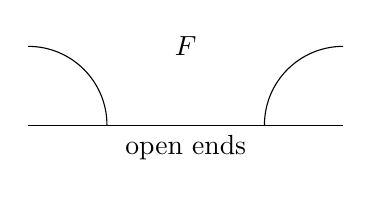
\begin{tikzpicture}
\draw (-2,0)--(2,0);
\draw (-1,0) arc (0:90:1);
\draw (1,0) arc (180:90:1);
\node at (0,1) {$F$};
\node at (0,0)[below] {open ends};
\end{tikzpicture}
\end{center}
\begin{center}
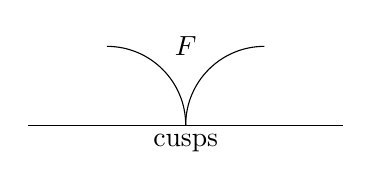
\begin{tikzpicture}
\draw (-2,0)--(2,0);
\draw (0,0) arc (0:90:1);
\draw (0,0) arc (180:90:1);
\node at (0,1) {$F$};
\node at (0,0)[below] {cusps};
\end{tikzpicture}
\end{center}

\begin{theorem}
$\Gamma\leq\SL_2(\mathbb R)$ is a discrete subgroup, $z_0\in\mathcal H$ is a non-elliptic point of $\Gamma$, $\mathcal F=\mathcal F(z_0)$ as above. The following are equivalent
\begin{enumerate}
\item $\mathcal F$ has finitely many sides and all ends on $\mathbb R\cup\{\infty\}$ are cusps
\item $\Vol(\mathcal F)$ is finite
\end{enumerate}
\end{theorem}

\begin{note}
The sides of $\mathcal F$ are the segments $L_\gamma$ of nonzero length
\end{note}

\begin{proof}
1.$\Rightarrow$2.: Follows from Lemma \ref{Lemma from Gauss-Bonet} \\
2.$\Rightarrow$1.: Finiteness follows from Lemma \ref{Lemma from Gauss-Bonet}. If there are open ends, then there will be infinitely many geodesic triangles in $F$ with vertices on $\mathbb RP^1$, each such triangle has area $\pi$ by Lemma \ref{Lemma from Gauss-Bonet}, so $\Vol(F)=\infty$ which is a contradiction
\begin{center}
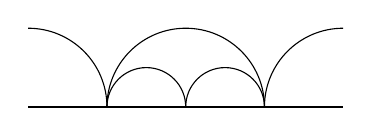
\begin{tikzpicture}
\draw (-2,0)--(2,0);
\draw (-1,0) arc (0:90:1);
\draw (1,0) arc (180:90:1);
\draw (1,0) arc (0:180:1);
\draw (0,0) arc (0:180:0.5);
\draw (0,0) arc (180:0:0.5);
\end{tikzpicture}
\end{center}
\end{proof}

\begin{lemma}\label{Lemma from Gauss-Bonet}
Let $P$ be a polygon on $\mathbb CP^1$ whose sides consists of $N$ geodesics. Let $\alpha_1,\cdots,\alpha_N$ be the interior angle at each vertex (we allow the vertex to be on $\mathbb R\cup\{\infty\}$), so the angle at such a vertex is 0), then $\Vol(P)=(N-2)\pi-\sum_{i=1}^N\alpha_i$. In particular, if $N=3$ and all 3 vertices are all on $\mathbb R\cup\{\infty\}$, then $\Vol(P)=\pi$
\end{lemma}

\begin{proof}
If all vertices are in $\mathcal H$, Gauss-Bonnet says
\[\int_Pkd\mu+\sum_{i=1}^N(\pi-\alpha_i)=2\pi\chi(P)\]
In this particular setting, $k\equiv-1$ is the constant curvature, $\chi(P)=1$ is the Euler characteristic. If there are cusps, truncate and take limit
\end{proof}

\begin{theorem}
Let $\Gamma$, $z_0$, $\mathcal F=\mathcal F(z_0)$ be as above. Suppose $\Vol(\mathcal F)<\infty$, then
\begin{enumerate}
\item Each of the (finitely many) cusps is a parabolic point for $\Gamma$, and not a hyperbolic point. Its stabilizer in $\overline\Gamma$ is isomorphic to $\mathbb Z$
\item There are finitely many elliptic points in $\mathcal F$, all lying on $\partial \mathcal F$
\item Each $\Gamma$-orbit of parabolic points of $\Gamma$ contains at least one cusp of $\mathcal F$
\end{enumerate}
\end{theorem}

\begin{proof}
\begin{enumerate}[label=\roman*]
\item 
\begin{enumerate}[label=\alph*)]
\item A cusp cannot be a hyperbolic point: Suppose not, then we may assume the cusp is at 0 and $\exists\gamma=\begin{bmatrix}
a&0 \\
0& a^{-1}
\end{bmatrix}\in\Gamma-\{\pm I\}$. Then $\gamma$ fixes the geodesic $(0,1\infty)$ and acts by fixes the geodesic $(0,i\infty)$ and acts by translation by a fixed hyperbolic distance on $(0,i\infty)$. Then any point on $(0,i\infty)$ can be moved to fixed segment $S$ on $(0,i\infty)$ by applying some power of $\gamma$. Let $z$ be an interior of $\mathcal F$. Then the geodesic from $z$ to 0 lie in the interior of $\mathcal F$, choose a sequence of points $z_n$ converging to 0 on this geodesic. Then we can find a sequence $w_n$ on $(0,i\infty)$ such that $d(z_n,w_n)\to0$ as $n\to\infty$. Apply some power of $\gamma$ to each $w_n$ to move them in $S$, then $z_n$ will be moved to accumulate near $S$ because $\gamma$ is an isometry. This contradicts local finiteness
\item Any cusp is a parabolic point ($\Rightarrow$ stabilizer in $\overline\Gamma$ isomorphic to $\mathbb Z$). Observation: If $\mathcal F$ and $\gamma(\mathcal F)$ have a common cusp $S$, then $\gamma^{-1}(S)$ is also a cusp of $\mathcal F$. $\forall$ cusp $S$ of $F$, there are infinitely many $\gamma\in\Gamma$ such that $S$ is also  a cusp of $\gamma(\mathcal F)$. If stabilizer of $s$ in $\Gamma$ is trivial, then there would be infinitely many cusps of $F$ by the above observation. This contradicts Theorem \ref{}. So stabilizer of $S$ in $\overline\Gamma$ is nontrivial and by 1a), $S$ is a parabolic point
\end{enumerate}
\item Elliptic points cannot lie in $\mathcal F^\circ$ since $\gamma(\mathcal F^\circ)\cap \mathcal F^\circ=\varnothing$ for any non-scalar $\gamma\in\Gamma$. They are either a vertex of $\mathcal F$ or mid-point of a side, hence finitely many
\item Assertion on parabolic points of $\Gamma$ will be proved later. It essentially boils down to Hausdorffness of the compactification of $\Gamma\backslash\mathcal H\cong \mathcal F/\sim$ by adding cusps
\end{enumerate}
\end{proof}

\begin{remark}
In fact part 3. suggests how to define compactification of $\Gamma\backslash\mathcal H$ without using any specific fundamental domain
\end{remark}

\subsection{Compactifying $\Gamma\backslash\mathcal H$}

Fix $\Gamma\leq \SL_2(\mathbb R)$ discrete subgroup. Let $P_\Gamma$ be the set of parabolic points of $\Gamma$ on $\mathbb R\cup\{\infty\}$($P_\Gamma=\varnothing$ if no parabolic points). Let $\mathcal H^*=\mathcal H^*_\Gamma=\mathcal H\cup P_\Gamma$.

\textbf{Goal} is to put a topology on $\mathcal H^*$, show that when $\Vol(\Gamma\backslash\mathcal H)<\infty$, $\Gamma\backslash\mathcal H^*$ is a nice compactification of $\Gamma\backslash\mathcal H$ and can be identified with a quotient of $\mathcal F^*=\mathcal F\cup\{\text{cusps of }\mathcal F\}$ where $\mathcal F$ is a fundamental domain for $\Gamma$ as above \\
For $l>0$, let $U_\infty(l)=\{z\in\mathcal H|\operatorname{Im} z>l\}$ and $U^*_\infty(l)=U_\infty(l)\cup\{\infty\}$, for $t\in\mathbb R$, let $U_t(l)=\sigma U_\infty(l)$, $U^*_t(l)=\sigma U^*_\infty(l)=U_t(l)\cup\{t\}$, where $\sigma\in\PSL_2(\mathbb R)$ is chosen so that $\sigma\infty=t$. The boundaries of $U_t(l)$ are horocycles at $t\in\mathbb R\cup\{\infty\}$. Define a topology on $\mathcal H^*$ so that $\mathcal H$ is an open subset, and $U^*_t(l)$ form a system of neighborhoods of $t\in\mathbb R\cup\{\infty\}$, then $\mathcal H^*$ is a second countable(since $\Gamma$ and hence $P_\Gamma$ is countable and Hausdorff), but not locally compact. $\Gamma$ acts continuously on $\mathcal H^*$, but not properly: stabilizes at $t\in P_\Gamma$ are isomorphic to $\mathbb Z$, infinite

\begin{example}
When $\Gamma=\SL_2(\mathbb Z)$, $P_\Gamma=\mathbb Q\cup\{\infty\}$. $\Gamma$ acts transitively on $P_\Gamma$ (an easy check, also follows from Theorem \ref{} and Theorem \ref{}, noticing that the standard fundamental domain for $\SL_2(\mathbb Z)$ has only one cusp $\infty$). $\overline\Gamma_\infty=\left\langle\begin{bmatrix}
1&1 \\
0&1
\end{bmatrix}\right\rangle$, $U^*_\infty(l)/\overline\Gamma_\infty$ is homeomorphic to an open disc
\end{example}

\begin{lemma}
For any $t\in P_\Gamma$, $\overline\Gamma_t\cong\mathbb Z$ and a generator has the form $\sigma\begin{bmatrix}
1&h \\
0&1
\end{bmatrix}\sigma^{-1}$ where $h>0$, $\sigma\in\SL_2(\mathbb R)$, $\sigma\infty=t$
\end{lemma}

\begin{proof}
We may assume $t=\infty$, then
\[\Gamma\subseteq\left\{\pm\begin{bmatrix}
*&* \\
0&*
\end{bmatrix}\right\}\]
Since $\infty\in P_\Gamma$, $\exists x>0$ such that $\begin{bmatrix}
1& x\\
0&1
\end{bmatrix}\in\Gamma_\infty\cdot\{\pm1\}$. If $\exists\begin{bmatrix}
a&0 \\
0&a^{-1}
\end{bmatrix}\in\Gamma_\infty$, may assume $|a|\leq1$, then
\[\begin{bmatrix}
a&0 \\
0&a^{-1}
\end{bmatrix}^n\begin{bmatrix}
1&x \\
0&1
\end{bmatrix}\begin{bmatrix}
a&0 \\
0&a^{-1}
\end{bmatrix}^{-n}=\begin{bmatrix}
1&a^{2n}x \\
0&1
\end{bmatrix}\in\Gamma\]
$\Gamma$ is discrete $\Rightarrow$ $a=\pm1$. $\Rightarrow\overline\Gamma_\infty$ is a discrete subgroup of $\left\{\begin{bmatrix}
1&* \\
0&1
\end{bmatrix}\right\}\cong\mathbb R\Rightarrow\overline\Gamma_\infty\cong\mathbb Z$
\end{proof}

\begin{lemma}
Suppose $\begin{bmatrix}
1&h \\
0&1
\end{bmatrix}\in\overline\Gamma$ for some $h\neq0$, let $\gamma=\begin{bmatrix}
a&b\\
c&d
\end{bmatrix}\in\Gamma$. If $|hc|<1$, then $c=0$
\end{lemma}

\begin{proof}[Miyake 1.7.3]
Define inductively $\gamma_n\in\Gamma\cdot\{\pm1\}$, $\gamma_0=\gamma$, $\gamma_{n+1}=\gamma_n\begin{bmatrix}
1&h \\
0&1
\end{bmatrix}\gamma_n^{-1}$, $|hc|<1$ implies $\gamma_n\xrightarrow{n\to\infty}\begin{bmatrix}
1&h \\
0&1
\end{bmatrix}$. $\Gamma$ discrete $\Rightarrow c=0$
\end{proof}

\begin{lemma}
For any compact subset $K\subseteq\mathcal H$, for any $s\in P_\Gamma$, $\exists l>0$ such that $K\cap\gamma U_s(l)=\varnothing$, $\forall\gamma\in\Gamma$ (Or equivalently, $\gamma(K)\cap U_s(l)=\varnothing$, $\forall\gamma\in\Gamma$)
\end{lemma}

\begin{proof}
Let $\sigma\in\SL_2(\mathbb R)$ with $\sigma\infty=s$, since $K$ is compact, $\exists0<l_1<l_2$ such that
\[\sigma^{-1}(K)\subseteq\{z\in\mathcal H|l_1<\operatorname{Im}(z)<l_2\}\]
Since $s$ is a parabolic point, $\exists h\neq0$ scuh that $\begin{bmatrix}
1&h \\
0&1
\end{bmatrix}\in\sigma^{-1}\Gamma\cdot\{\pm1\}\sigma$. Let $l=\max\{h^2/l_1,l_2\}$. Let $\gamma\in\Gamma$ and denote $\delta=\sigma^{-1}\gamma\sigma=\begin{bmatrix}
a&b \\
c&d
\end{bmatrix}$. If $c=0$, then $\delta U_\infty(l)\cap\sigma^{-1}K=U_\infty(l)\cap\sigma^{-1}K=\varnothing$. If $c\neq0$, then by Lemma \ref{}, $|hc|\geq1$ $\Rightarrow z\in U_\infty(l)$
\[\operatorname{Im}(\delta z)=\frac{\operatorname{Im}z}{|cz+d|^2}\leq\frac{1}{c^2\operatorname{Im}z}<\frac{1}{c^2l}\leq\frac{h^2}{l}\leq l_1\]
$\Rightarrow\delta U_\infty(l)\cap\sigma^{-1}K=\varnothing$. Thus $\gamma U_s(l)\cap K=\gamma\sigma U_\infty(l)\cap K=\sigma(\delta U_\infty(l)\cap\sigma^{-1}K)=\varnothing$
\end{proof}

\begin{lemma}
Let $s,t\in P_\Gamma$, then $\forall l>0$, $\exists l'>0$ such that $\forall\gamma\in\Gamma$, if $\gamma s\neq t$, then $\gamma U_s(l)\cap U_t(l')=\varnothing$
\end{lemma}

\begin{proof}
Let $\sigma\in\SL_2(\mathbb R)$ with $\sigma\infty=s$, since $s\in P_\Gamma$, $\exists h\neq0$ such that
\[\delta=\sigma\begin{bmatrix}
1&h \\
0&1
\end{bmatrix}\sigma^{-1}\in\Gamma_s\cdot\{\pm1\}\subseteq\Gamma\cdot\{\pm1\}\]
Let $K=\{z\in\mathcal H|\operatorname{Im}z=l,0\leq\operatorname{Re}z\leq|h|\}$, by Lemma \ref{}, $\exists l'>0$ such that $\gamma\sigma(K)\cap U_t(l')=\varnothing$, $\forall \gamma\in\Gamma$. Let $\gamma\in\Gamma$ with $\gamma s=t$. Suppose $\gamma U_s(l)\cap U_t(l')\neq\varnothing$, then $\gamma(\partial U_s(l)-\{s\})\cap U_t(l')\neq\varnothing$ since $\gamma s\neq t$. $\Rightarrow$ for some $n\in\mathbb Z$, $\gamma\delta^n\sigma(K)\cap U_t(l')\neq\varnothing$ is a contradiction
\end{proof}

\begin{corollary}
$\forall s\in P_\Gamma$, $\exists C>0$ such that $\overline\Gamma\backslash U^*_s(l)\to\Gamma\backslash\mathcal H^*$ is an open embedding for any $l>C$
\end{corollary}

\begin{proof}
Take $s=t$ in Lemma \ref{}, we see that for $l>>0$, $\{\gamma\in\overline\Gamma|\gamma U_s(l)\cap U_s(l)\neq\varnothing\}=\overline\Gamma_s$
\end{proof}

\begin{corollary}
$\Gamma\backslash\mathcal H^*$ is locally compact Hausdorff
\end{corollary}

\begin{proof}
Corollary \ref{} $\Rightarrow$ locally compact since $\overline\Gamma_s\backslash\overline{U^*_s(l)}$ is compact. (Exercise: check this and also check that $\overline{U^*_s(l)}$ is not compact). From previous note, $\Gamma\backslash\mathcal H$ is Hausdorff, the rest follows from Lemma \ref{} and Lemma \ref{}
\end{proof}

Finally we can finish the proof of Theorem \ref{} 3. Suppose $s\in P_\Gamma$ and the orbit $\Gamma s$ does not contain any cusp of $F$. Fix a neighborhood $U=U^*_s(l)$ of $s$. The hypothesis $\Vol(F)<\infty$ implies that $F$ has only finitely many cusps: $\{s_1,\cdots,s_n\}$ (by Theorem \ref{}). By Lemma \ref{}, there exist neighborhoods $U_i$ of $s_i$ such that $\gamma U\cap U_i=\varnothing$, $\forall\gamma\in\Gamma$, $\forall 1\leq i\leq n$. By Lemma \ref{}, we can shrink $U$ so that it does not intersect the compact set $K=\mathcal F-\bigcup_{i=1}^nU_i$. Then $\gamma U\cap F=\varnothing$, $\forall \gamma\in\Gamma$, contradicting the definition of fundamental domain. Thus $\Gamma s$ contains some cusps of $F$

\begin{remark}
Suppose $\Vol(\mathcal F)<\infty$. Let $\mathcal F^*$ be the closure of $\mathcal F$ in $\mathcal H\cup\mathbb R\cup\{\infty\}$, then $\mathcal F^*=\mathcal F\cup\{\text{cusps}\}$ and $\mathcal F^*/\sim$ is homeomorphic to $\Gamma\backslash\mathcal H^*$
\end{remark}

\begin{definition}[Riemann surface structure on $\Gamma\backslash\mathcal H^*$]
$\forall z\in\mathcal H^*=\mathcal H\cup P_\Gamma$, let $U_z$ be an open neighborhood of $z$ such that $\{\gamma\in\Gamma|\gamma U_z\cap U_z\neq\varnothing\}=\Gamma _z$. Existence of $U_z$ follows from Proposition \ref{} in previous note, when $z\in\mathcal H$, and Lemma \ref{} (or corollary \ref{}) when $z\in P_\Gamma$. Then $\Gamma_z\backslash U_z\to\Gamma\backslash\mathcal H^*$ is an open embedding for any $z\in\mathcal H^*$. We use $\{\Gamma_z/U_z,\phi_z\}_{z\in\mathcal H^*}$ as coordinate charts, $\phi_z$ is to be defined
\begin{enumerate}
\item If $z\in\mathcal H$ is a non-elliptic point, then $\overline\Gamma_z=\{1\}$, let $\phi_z:\Gamma_z\backslash U_z\to U_z$ be the natural homeomorphism
\item If $z\in\mathcal H$ is elliptic, then $\overline\Gamma_z$ is a cyclic group of order $n>1$. Let $\lambda:\mathcal H\to\mathbb D$ be an isomorphism of complex manifold such that $\lambda(z)=0$. By Schwarz lemma, $\lambda\overline\Gamma_z\lambda^{-1}$ is the group generated by $\frac{2\pi}{n}$ rotation. Define $\phi_z:\Gamma_z\backslash U_z\to\mathbb C$ by $\phi_z(w)=\lambda(w)^n$ \begin{center}
\begin{tikzcd}
U_z \arrow[r, hook] \arrow[d]               & \mathcal H \arrow[r, "\lambda"] & \mathbb D \arrow[d, "u\mapsto u^n"] \\
\Gamma_z\backslash U_z \arrow[rr, "\phi_z"] &                                 & \mathbb D                          
\end{tikzcd}
\end{center}
\item If $s\in P_\Gamma$ is parabolic, then by Lemma \ref{}, \[\sigma^{-1}\overline\Gamma_s\sigma=\left\langle\begin{bmatrix}
1&h \\
0&1
\end{bmatrix}\right\rangle\cong\mathbb Z\]Where $h>0$, here $\sigma\in\SL_2(\mathbb R)$, $\sigma\infty=s$, define $\phi_s(w)=\exp(\frac{2\pi i}{h}\sigma^{-1}(w))$ \begin{center}
\begin{tikzcd}
U_s \arrow[r, "\sigma^{-1}"] \arrow[d]     & \mathcal H\cup\{\infty\} \arrow[d, "\exp(\frac{2\pi i}{h}z)"] \\
\Gamma_s\backslash U_s \arrow[r, "\phi_s"] & \mathbb D                                                    
\end{tikzcd}
\end{center}
\end{enumerate}
\end{definition}

Let's write $X(\Gamma)=\Gamma\backslash\mathcal H^*$, $Y(\Gamma)=\Gamma\backslash\mathcal H$. Riemann surfaces with complex structures defined above. $X(\Gamma)-Y(\Gamma)$ is a discrete set of cusps of $X(\Gamma)$

\begin{theorem}[Siegel]
$X(\Gamma)$ is compact $\iff$ $Y(\Gamma)$ has finite volume
\end{theorem}

\begin{proof}
$\Rightarrow:$ $X(\Gamma)$ compact $\Rightarrow$ finitely many cusps, a neighborhood of each cusp has finite volume
\[\int_l^\infty\int_0^h\frac{dxdy}{y^2}=h\int_l^\infty\frac{dy}{y^2}<\infty\]
$\Leftarrow:$ Let $\mathcal F$ be the fundamental domain as in Theorem \ref{}, then $\Vol(\mathcal F)=\Vol(Y(\Gamma))<\infty$ $\Rightarrow$ $X(\Gamma)\approx \mathcal F^*/\sim$ is compact by Theorem \ref{}. Here $\mathcal F^*=\mathcal F\cup\{\text{cusps}\}$ is viewed as a closed subset of $\mathbb{CP}^1$, hence compact
\end{proof}

\end{document}